
\section{Proposed System}

\begin{figure}[h]
\noindent
\begin{minipage}{\textwidth}
\makebox[\textwidth]{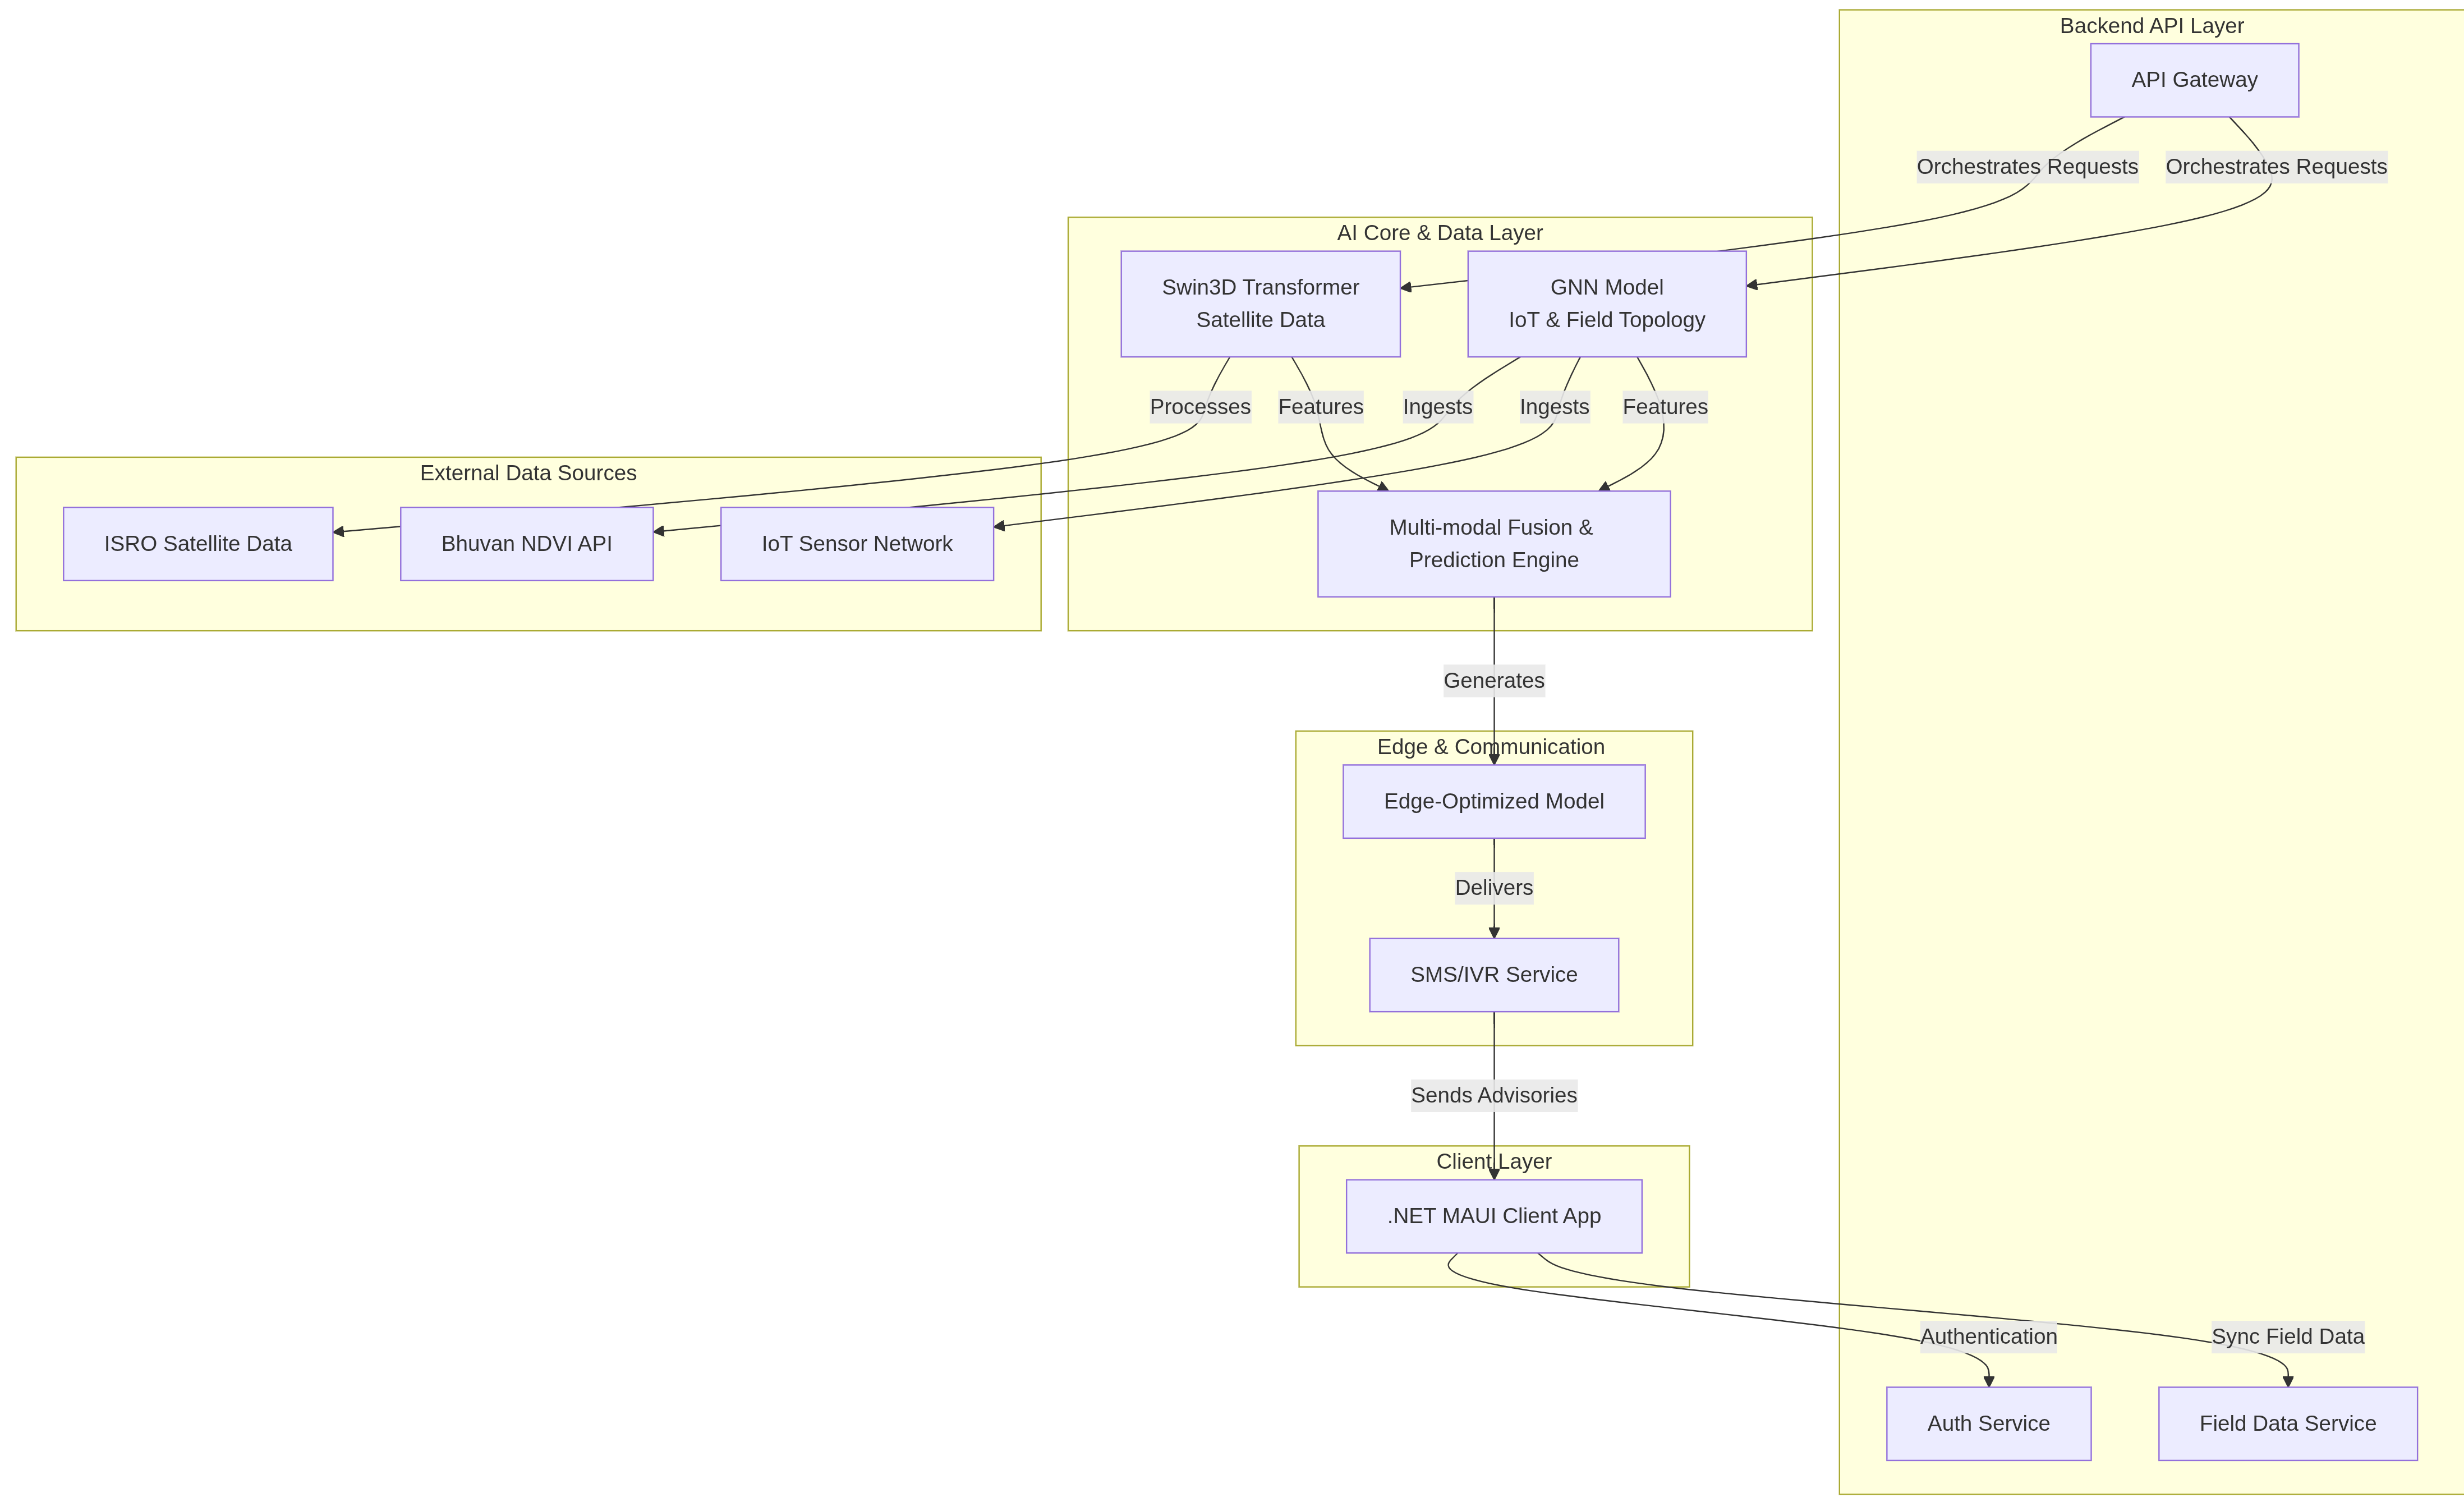
\includegraphics[width=1.15\textwidth]{Images/proposed_system.png}}
\caption{Proposed system architecture.}
\label{fig:proposed_system}
\end{minipage}
\end{figure}

This research proposes a comprehensive AI-powered system for village-level crop yield forecasting and farmer advisory services. The system integrates advanced machine learning models with practical technology delivery to support agricultural decision-making.

Our solution employs a multi-layered architecture that combines AI processing with accessible farmer interfaces. The system collects data from multiple sources, processes it through specialised AI models, and delivers actionable insights to end-users through both mobile applications and basic feature phones.

The system gathers agricultural data from three primary sources:
\begin{itemize}
    \item High-resolution satellite imagery from ISRO for temporal analysis.
    \item IoT sensor networks deployed across farm fields for real-time monitoring.
    \item Bhuvan NDVI API data for vegetation health assessment.
\end{itemize}

The proposed system features an AI-powered prediction engine that leverages a multi-modal data fusion approach. For temporal analysis, Swin3D Transformers \cite{liu2022swin3d} process satellite time-series data to model crop growth patterns, while Graph Neural Networks \cite{brody2022gatv2} capture spatial relationships and environmental dependencies between neighbouring fields. These models are fused to generate high-accuracy yield predictions. To ensure broad accessibility, an edge-optimised advisory system compresses the predictive model for low-end hardware deployment. Finally, a farmer interaction platform --- including a .NET MAUI cross-platform application and inclusive communication channels such as SMS and Interactive Voice Response (IVR) --- delivers personalised advisories, effectively bridging the digital divide for rural communities.

The system's design specifically addresses the challenge of technology accessibility in rural environments, making advanced agricultural insights available to farmers regardless of their access to sophisticated hardware or digital literacy levels.
